\documentclass[11pt, a4paper]{article}

% --- PAQUETES ESENCIALES ---
\usepackage[utf8]{inputenc}
\usepackage[T1]{fontenc}
\usepackage[spanish,es-tabla]{babel} % es-tabla mejora los nombres de las tablas
\usepackage[margin=2.5cm]{geometry} % Margen estándar de 2.5cm
\usepackage{amsmath}
\usepackage{amssymb}
\usepackage{graphicx}   % Para imágenes
\usepackage{booktabs}   % Para tablas profesionales (usado en Carta Gantt)
\usepackage{caption}    % Para mejores captions
\usepackage{float}      % Para mejor control de la posición de figuras [H]
\usepackage{parskip}    % Pone un espacio entre párrafos en lugar de indentación

\captionsetup{format=hang, justification=justified, singlelinecheck=false, labelfont=bf}

% --- PAQUETE PARA BIBLIOGRAFÍA (NUMÉRICA TIPO ISO) ---
\usepackage[backend=biber, style=numeric, sorting=none]{biblatex}
\addbibresource{bibliografia.bib} % Archivo que contendrá las referencias
% --- PAQUETE PARA HIPERVÍNCULOS ---
\usepackage{hyperref}
\hypersetup{
    colorlinks=true,
    linkcolor=black, % Color de enlaces internos (TOC, figuras)
    urlcolor=blue,   % Color de enlaces web
    citecolor=black, % Color de las citas bibliográficas [1]
}

% --- CONFIGURACIÓN GENERAL ---
\graphicspath{ {./images/}} % Carpeta donde guardas las imágenes


\begin{document}

% --- PÁGINA DE TÍTULO ---
\begin{titlepage}
    \centering
    % Logo y Nombre de la Universidad
    
\includegraphics[width=4cm]{usach.png}\\[2cm]
    \textsc{\LARGE Universidad de Santiago de Chile}\\[0.5cm]
    \textsc{\Large Facultad de Ingeniería}\\[0.5cm]
    \textsc{\Large Departamento de Ingeniería Mecánica}\\[2.5cm]
    
    % Título del Informe
    \rule{\textwidth}{1.5pt}\vspace{0.4cm}
    {\Huge \bfseries Informe de Proyecto: \\[0.5cm] Diseño y Mejora de Compás de Trazado Industrial}\\[0.4cm]
    \rule{\textwidth}{1.5pt}\\[1.5cm]
    
    % Asignatura
    {\Large \textit{Introducción a la Ingeniería - Sección Dibujo de Ingeniería}}\\[2cm]
    
    % Autores
    \begin{minipage}{0.4\textwidth}
        \begin{flushleft} \large
            \textbf{Autor:}\\
            Lukas Espinoza
        \end{flushleft}
    \end{minipage}
    \begin{minipage}{0.4\textwidth}
        \begin{flushright} \large
            \textbf{Profesor:}\\
            Paulina Bravo
        \end{flushright}
    \end{minipage}

    \vfill % Empuja la fecha al final de la página
    
    % Fecha
    {\large \today}
\end{titlepage}

% --- RESUMEN EJECUTIVO ---
\begin{abstract}
    \noindent \textbf{Resumen} \\
    Este informe detalla el proceso de diseño para la mejora de un compás de trazado industrial, un instrumento de precisión utilizado en talleres mecánicos. El proyecto aborda las limitaciones de los modelos actuales, como la falta de rigidez y la dificultad de ajuste fino. Se propone un nuevo diseño que incorpora [mencionar 1 o 2 mejoras clave, ej: un mecanismo de tornillo sin fin para el ajuste y brazos reforzados]. El desarrollo incluye el análisis de mecanismos de referencia, la creación de un boceto inicial, la planificación de tareas mediante una carta Gantt y la elaboración de planos técnicos completos (conjunto, despiece y fabricación) utilizando AutoCAD, siguiendo la normativa chilena de dibujo técnico.
\end{abstract}

\newpage
\tableofcontents
\newpage

\section{Introducción y Problemática}
\subsection{Descripción del problema}
El trazado de precisión sobre superficies metálicas es una tarea fundamental en la fabricación mecánica. Los compases de trazado convencionales a menudo presentan problemas de flexión en sus brazos al aplicar la fuerza necesaria para marcar el material, lo que resulta en una pérdida de precisión. Adicionalmente, el sistema de ajuste por fricción puede ser impreciso y propenso a desajustarse durante el uso.

Este proyecto tiene como objetivo diseñar una mejora a un compás industrial, abordando directamente estas deficiencias. El alcance se limita al diseño mecánico y la representación gráfica de las piezas, sin incluir análisis de elementos finitos o la construcción de un prototipo físico. Las limitaciones incluyen el uso de materiales estándar como acero y aluminio, y el diseño de un máximo de [ej: 7] piezas fabricables.

\section{Mecanismos de Referencia}
Para el desarrollo de la propuesta, se analizaron dos mecanismos principales que inspiran las mejoras.

El primer mecanismo de referencia, mostrado en la Figura \ref{fig:ref1}, es un compás de alta precisión de la marca Starrett \cite{starrett_compass}. Se eligió este modelo por su robusto sistema de articulación y su tornillo de ajuste rápido, que sirven como base para mejorar la rigidez del conjunto.

\begin{figure}[H]
    \centering
    \includegraphics[width=0.6\textwidth]{referencia1.png} % Cambiar 'referencia1.png' por tu imagen
    \caption{Compás de precisión Starrett Modelo 92 con ajuste por resorte \cite{starrett_compass}.}
    \label{fig:ref1}
\end{figure}

La segunda referencia, visible en la Figura \ref{fig:ref2}, es un sistema de ajuste micrométrico utilizado en calibradores \cite{pytel_dinamica}. Este principio de tornillo sin fin se adaptará para permitir un ajuste fino y estable de la apertura del compás, una característica clave de nuestra propuesta.

\begin{figure}[H]
    \centering
    \includegraphics[width=0.6\textwidth]{referencia2.png} % Cambiar 'referencia2.png' por tu imagen
    \caption{Detalle de un mecanismo de ajuste fino basado en tornillo \cite{pytel_dinamica}.}
    \label{fig:ref2}
\end{figure}

\section{Propuesta de Diseño y Boceto Inicial}
Nuestra propuesta consiste en un compás de brazos reforzados con una sección transversal en "I" para maximizar la rigidez. La articulación principal se rediseña para minimizar el juego, y se integra un sistema de ajuste fino mediante un tornillo moleteado que acciona una cremallera en uno de los brazos.

El boceto inicial del concepto se presenta en la Figura \ref{fig:boceto}. Este croquis muestra las dimensiones generales y la disposición de los componentes principales.

\begin{figure}[H]
    \centering
    \includegraphics[width=0.7\textwidth]{boceto.png} % Cambiar 'boceto.png' por tu imagen
    \caption{Boceto inicial del compás de trazado mejorado con dimensiones generales en milímetros.}
    \label{fig:boceto}
\end{figure}

\subsection{Análisis de Ventajas y Desventajas}
\subsubsection{Ventajas}
\begin{itemize}
    \item \textbf{Mayor Precisión:} El sistema de ajuste fino permite un control exacto de la apertura.
    \item \textbf{Rigidez Mejorada:} Los brazos reforzados evitan la flexión durante el trazado.
    \item \textbf{Durabilidad:} El diseño robusto asegura una mayor vida útil del instrumento.
\end{itemize}

\subsubsection{Desventajas}
\begin{itemize}
    \item \textbf{Mayor Costo de Fabricación:} El mecanismo de ajuste es más complejo que un sistema de fricción simple.
    \item \textbf{Peso Ligeramente Superior:} El refuerzo en los brazos podría incrementar el peso total del instrumento.
\end{itemize}

\section{Planificación del Proyecto (Carta Gantt)}
La distribución de tareas para la realización de este proyecto se detalla en la Tabla \ref{tab:gantt}.

\begin{table}[H]
    \centering
    \caption{Asignación de actividades del proyecto.}
    \label{tab:gantt}
    \begin{tabular}{@{}lll@{}}
        \toprule
        \textbf{Actividad} & \textbf{Responsable} & \textbf{Estado} \\
        \midrule
        Investigación de problemática y mecanismos de referencia & Lukas Espinoza & Completado \\
        Creación de boceto inicial y definición de la propuesta & Lukas Espinoza & Completado \\
        Dibujo de piezas en AutoCAD (Planos de fabricación) & Lukas Espinoza & En Progreso \\
        Ensamblaje virtual y creación de plano de conjunto & Lukas Espinoza & Pendiente \\
        Creación de plano de despiece y lista de piezas & Lukas Espinoza & Pendiente \\
        Redacción del informe y formato final & Lukas Espinoza & En Progreso \\
        \bottomrule
    \end{tabular}
\end{table}

\section{Resultados: Planos del Mecanismo}
En esta sección se presentan los planos técnicos del diseño, generados en AutoCAD y cumpliendo con la normativa de dibujo técnico correspondiente.
    
\subsection{Plano de Conjunto}
La Figura \ref{fig:conjunto} muestra el ensamblaje completo del compás, identificando cada componente con su respectivo número de marca.

\begin{figure}[H]
    \centering
    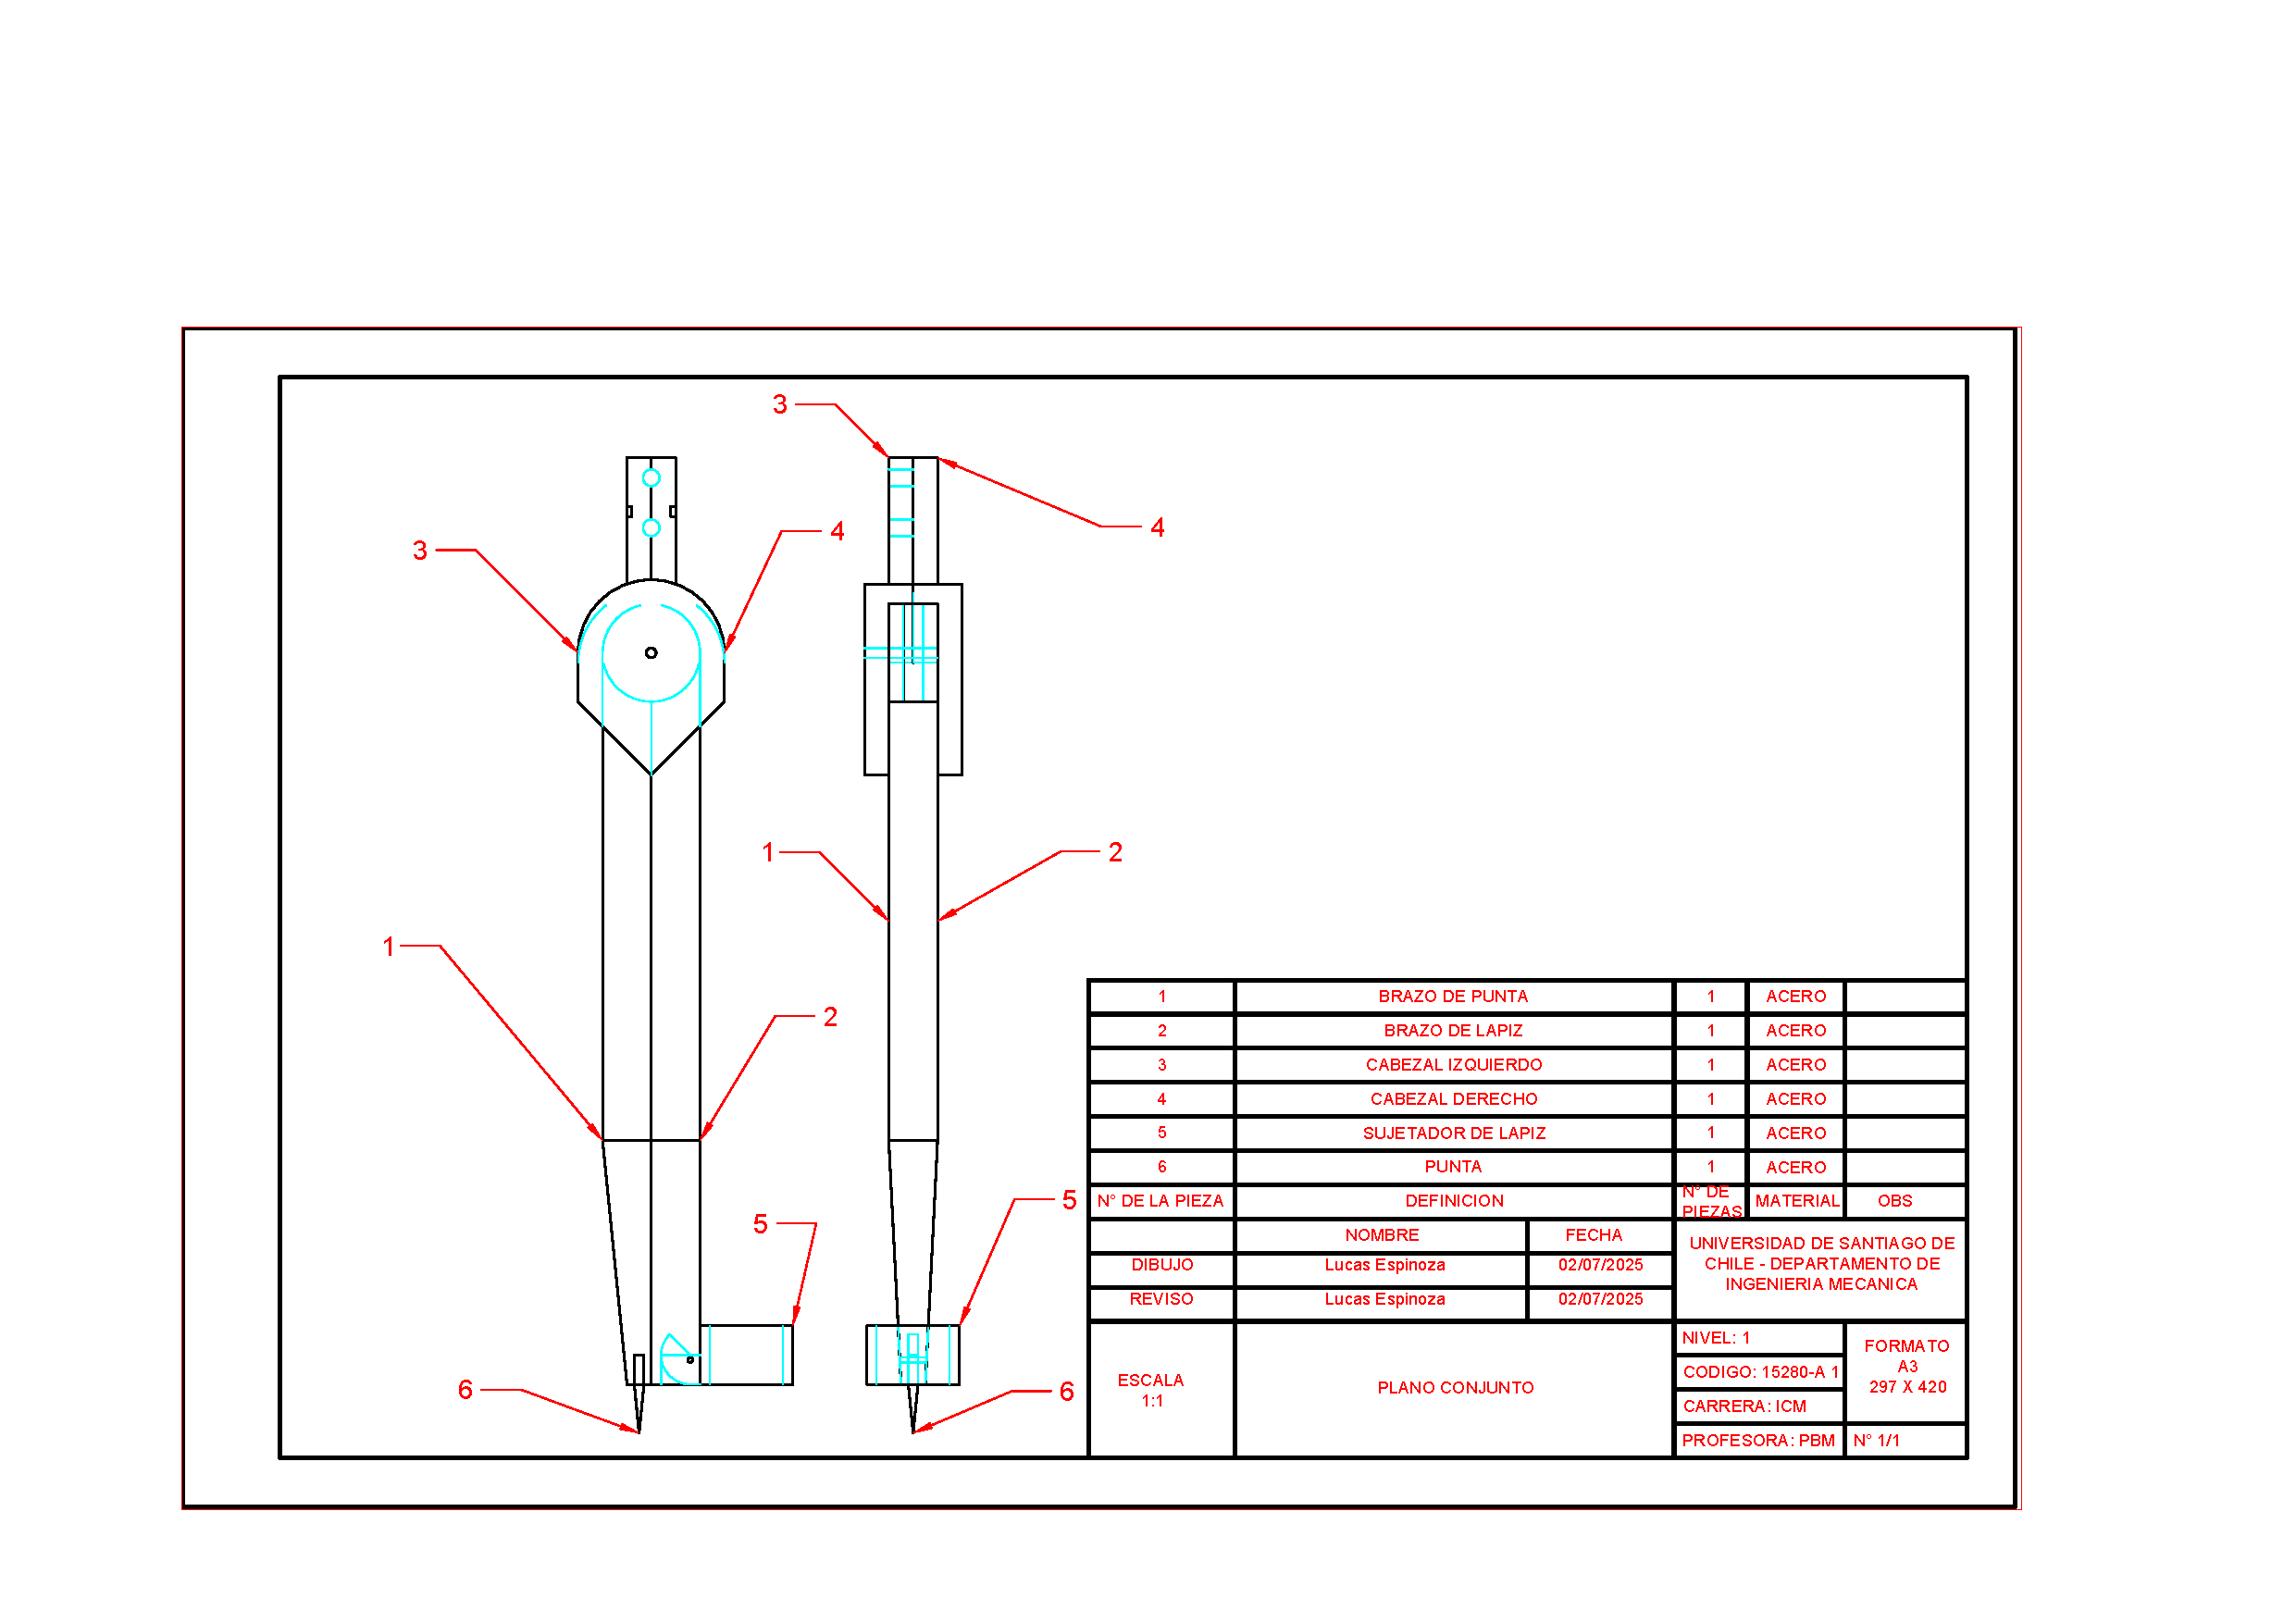
\includegraphics[width=\textwidth, height=20cm, keepaspectratio]{plano_conjunto.png}
    \caption{Plano de conjunto del compás de trazado mejorado.}
    \label{fig:conjunto}
\end{figure}

\subsection{Plano de Despiece}
El plano de despiece (Figura \ref{fig:despiece}) presenta una vista explosionada del mecanismo, facilitando la comprensión del ensamblaje y la relación entre las piezas. Incluye la lista de materiales (BOM).

\begin{figure}[H]
    \centering
    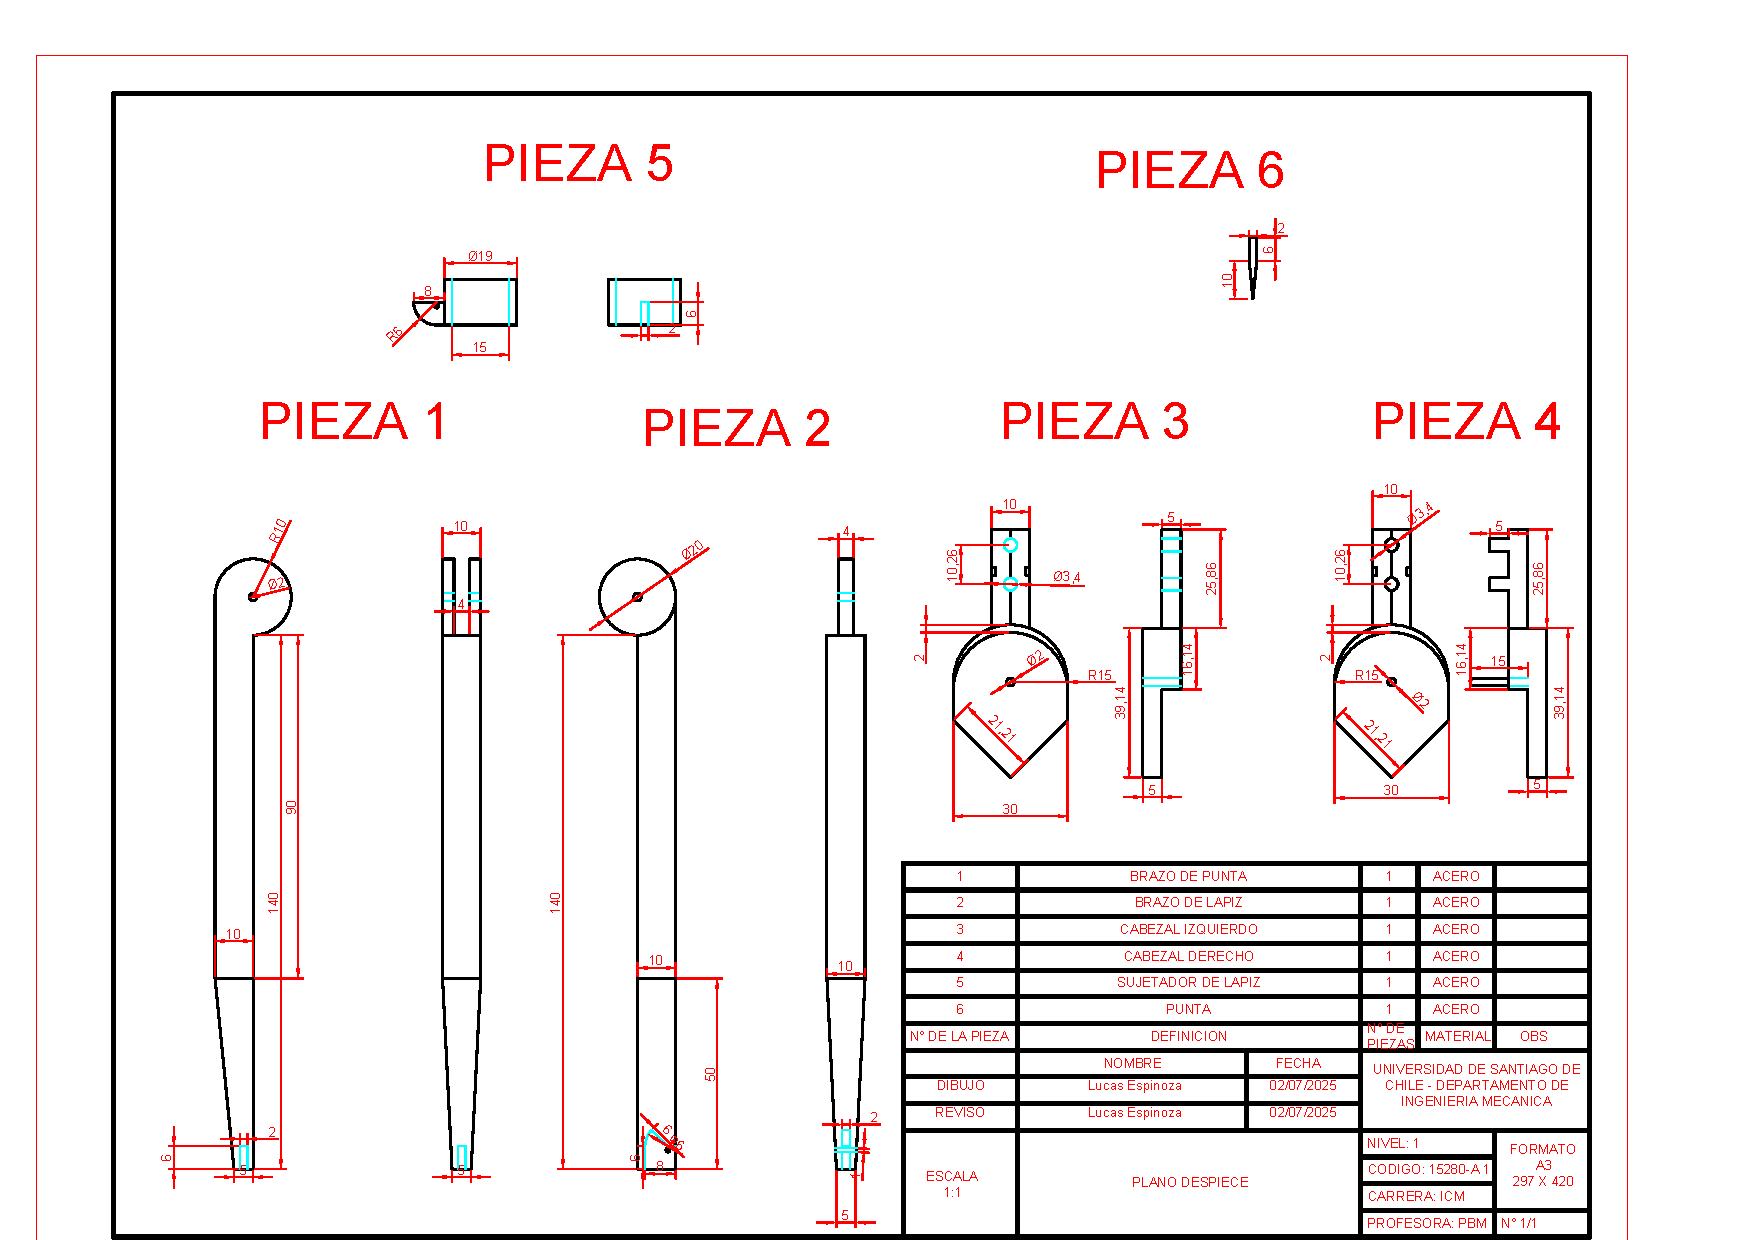
\includegraphics[width=\textwidth, height=20cm, keepaspectratio]{plano_despiece.png}
    \caption{Plano de despiece del compás.}
    \label{fig:despiece}
\end{figure}

\subsection{Planos de Fabricación}
A continuación, se adjuntan los planos de fabricación individuales para las piezas diseñadas. Por ejemplo, la Figura \ref{fig:fabricacion} muestra el plano del brazo principal.

\begin{figure}[H]
    \centering
    \includegraphics[width=\textwidth, height=20cm, keepaspectratio]{plano_fabricacion_pieza1.png}
    \caption{Plano de fabricación del Brazo Principal (Pieza 01).}
    \label{fig:fabricacion}
\end{figure}

\newpage
% --- BIBLIOGRAFÍA ---
\printbibliography[title={Referencias Bibliográficas}]

\end{document}
